\subsection{Physical Oceanography}

% \begin{wrapfigure}{!h}{3.7in}
\begin{figure}[!th]
  % \vspace{-0.5cm} 
  \centering 
  \subfigure[Predictions of currents and temperature at 10m depth from
  a \texttt{HOPS} (Harvard Ocean Prediction System) model with
  assimilation of temperature and salinity measurements collected by
  CTD profiles and
  current-meters.]{\label{fig:model}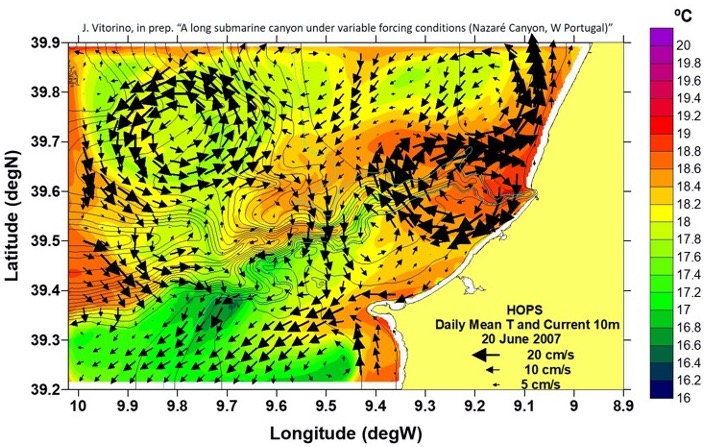
\includegraphics[scale=0.35]{fig/model.jpeg}}
  % \hspace{0.25cm}
  \subfigure[MUR SST image for June 20\textsuperscript{th} 2007. The
  red rectangle covers the area to be modeled in
  HOPS.]{\label{fig:SST}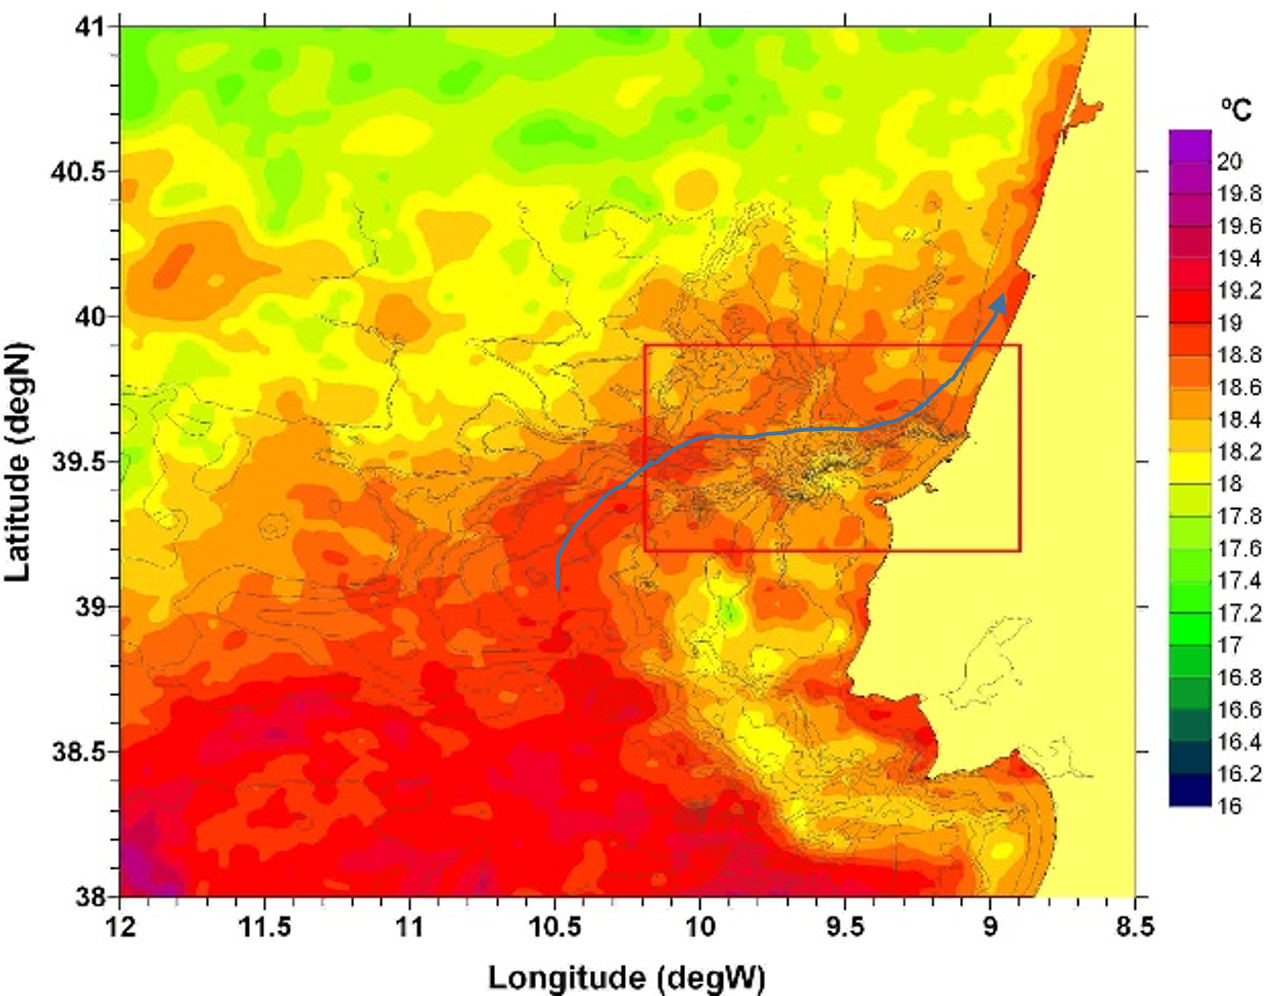
\includegraphics[scale=0.35]{fig/SST-Nazare.png}}
  \caption{}
% \vspace{-1cm}
% \end{wrapfigure}
\end{figure}

The geographical domain on which \proj will focus on, constitutes a
key area for the shaping of several main characteristics of the
shelf/slope oceanography of the northwestern Portuguese and Spanish
land-mass.  The important changes in the continental margin topography
that characterize this area lead to processes that impact not only the
local coastal environment but also, in what is still poorly understood,
the wider domain that extends to the north.

% The marked changes in the continental margin topography Finisterre
% that characterize this area play an important role in establishing the
% nature of the shelf response to wind forcing or the adjustment of the
% poleward slope intensified flow. The area (Fig. \ref{fig:model}) shows
% several expressive examples of coastal mesoscale features such as the
% large upwelling filament of Cabo Carvoeiro which is one of the larger
% and more persistent features of the summer upwelling regime in the
% western portuguese coast, with an expression similar to the large
% filaments off of Cape Finisterre (northwestern Spanish coast), Cape da
% Roca (near Lisbon) or Cape S.Vicente (in the southwestern tip of
% Portugal).

The area hosts important coastal meso-scale features such as the
upwelling filament of Cape Carvoeiro (Penich) that extends for more
than 200km. This is a recurrent feature of the summer upwelling regime
along the western Iberian coast together with the large filaments off
Cape Finisterre in the northwestern Spanish coast, of Cape da Roca in
the area near Lisbon or of Cape S\~{a}o Vicente in the southwestern
tip of Portugal \cite{haynes93}.

A rich variety of other coastal meso-scale and sub meso-scale
processes are linked to the presence of the \naz canyon. Among these,
\proj will focus on processes that:

\begin{itemize}[noitemsep,topsep=0pt,parsep=0pt,partopsep=0pt]

\item manifest in a relatively small geographical area; this would
  allows us to show the full potential of autonomous platform
  measurements in providing a detailed understanding of the processes

\item impact the local ecosystems; which bring together the physical,
  chemical and biological observations in a systematic manner and
  build a basis to support local fisheries and management of protected
  areas

\item potentially extend their influence to a broader area, shaping
  the conditions observed along the northwestern Portuguese margin; in
  this manner the local observations conducted in \proj will also
  contribute to a better understanding of the conditions prevailing in
  the wider region

\item are relevant for the operational support to navy operations or
  during crises at sea

\end{itemize}  

% The long and narrow \naz Canyon in addition promotes a rich variety of
% coastal mesoscale and submesoscale processes that not only directly
% affect the local ecosystems but can also contribute to impact a much
% larger coastal ocean area. Since they are linked to the canyon
% dynamics these processes develop on a relatively small area of the
% coastal ocean which are associated with specific areas of the canyon
% topography. In this way a strategy that concentrates several
% observation systems in this small area can bring considerable insight
% on the nature of the processes. This concentration is of particular
% interest for \proj objectives. \kc{TO BE CONTINUED...\ldots}
 
Two categories of processes that conform to the above requirements
will be the object of \proje's attention and are described below. The
exact nature of the processes to be covered during the field
experiment will depend on the period of the year during which the
experiment will take place (see Section \ref{sec:atsea-ops}) and on
the prevailing forcing conditions that affect the \naz canyon area
during the operational window of the experiment.

% \begin{description}
  
\paragraph{Process Category 1} Localized areas of intensified
upwelling and biological development promoted by the canyon.

Some important processes relate to the interaction of the shelf and
slope circulation with the canyon topography during periods of
favorable upwelling wind forcing. The basic mechanism for the response
of a narrow canyon to these type of forcing conditions is well known
-- namely the breakdown of geostrophy when the upwelling jet passes
over the abrupt canyon topography which promotes an up-canyon
circulation and with it, the intensification of the upwelling of cold,
nutrient rich subsurface waters at the canyon head
\cite{klinck96,she00}. Advection by the upwelling jet, displaces the
area of upward motion and nutrient intake in the upper layers to the
leeward flank of the canyon and adjacent shelf allowing this influence
to affect a large shelf area. In long submarine canyons in addition,
other processes come into play to prime the persistence of upwelling
conditions even when forcing decays, which lead to seasonal upwelling
conditions instead of an event-driven response
\cite{allen00,waterhouse09}.

The expression of these processes in the \naz canyon is however much
more complex and depends on the maturity of upwelling
conditions. During the early stages of the upwelling season or during
isolated upwelling events in the shelf away from the canyon, the
response to wind forcing is concentrated in the inner and mid
shelf. The water source from upwelling comes from relatively shallow
depths over the shelf below the \emph{Ekman layer} and the upwelling
conditions are very depended on the variability of the wind forcing
and can rapidly decay if favorable winds weaken.  During such types of
conditions previous observations suggest that the response of the \naz
canyon was consistent with the general mechanism described above, with
upwelling of cold and nutrient rich waters occurring along the
southern flank of the canyon and affecting the shelf to the south of
the canyon head.
 
\textsf{Specific Scientific Question 1:} if one of the periods
described above is covered during the \proj field program we will take
advantage of the combination of high resolution observations and data
assimilation models to get unparalleled insight into the physical,
chemical and biological processes that play together in the
intensified upwelling at the canyon head. Given the position of the
canyon head very near the coast, the study will also focus the
interaction of these processes with the littoral environment. In
addition, if the period of observation covers an upwelling condition
that occurs during winter or early spring, an associated focus of
interest will be to understand the impact of the circulation
associated with the canyon, in the retention of fish larvae and
eggs. In other areas of the shelf, the offshore transport promoted by
upwelling leads to dispersion of eggs and larvae to the outer shelf
and open ocean. This leads to negative impacts on fish stocks. In the
canyon area, the closed circulation cells that develop, can mitigate
the consequence of this offshore transport.

A different picture emerges during more mature phases of the upwelling
that develop when favorable winds persist for a few months. This is
typically the case at the end of the summer upwelling season (by
August and September) but can develop earlier in the year if the
previous winter conditions were marked by a positive phase of the
winter NAO (and prevailing upwelling favorable northerly winds). Away
from the canyon, the persistent upwelling favorable forcing builds an
upwelling response that now extends to the complete water column over
the shelf, expressed by an upward lift of isopycnics affecting the
first 200m depth or more. The source water for upwelling now comes
from depths of 200--300m over the upper slope. Although the surface
levels respond rapidly to the wind forcing and a decay or inversion of
the upwelling favorable winds can lead to the suppression of upwelling
conditions at near surface depths, this response does not remove the
expression of upwelling below. Consequently with the re-establishment
of the upwelling favorable forcing, the mature upwelling conditions
are re-established very rapidly. These are characterized by cold
upwelled waters extending over the complete continental shelf and the
upwelling front and jet being located over the outer shelf/upper slope
region.

During these periods, the upwelling jet intersects the \naz canyon
further offshore, primarily in the outer part of the upper canyon
section. The canyon topography and the blocking effect due to the
ridge between Cape Carvoeiro and Berlengas Islands, both contribute to
deflecting the upwelling jet towards the southern flank of the
canyon. At this location marked expressions of the impact of the jet
were observed in physical and biological measurements from previous
field experiments in this environment. 

 
\textsf{Specific Scientific Question 2:} If the \proj field program
takes place during a mature stage of upwelling such as the one
described above, we want to understand what processes take place in
this area along the southwestern flank of the upper \naz canyon. In
particular we want to evaluate how these processes are affecting the
marine ecosystems of the Berlengas archipelago, a marine protected
area.

\par

\paragraph{Process Category 2} Closed circulation cells promoted by
the canyon during wind forcing transitions.

Marked closed circulation cells are observed over the canyon
topography, near the canyon head during periods of decay or inversion
of the wind forcing conditions. These closed circulations are
associated with the inner canyon circulation and vertical motion near
the canyon head that was established in the canyon during periods
of active forcing and that persist after the decay of the forcing
conditions and are no longer advected by the shelf circulation. The
importance of these cells relies on their potential for confinement of
nutrient fluxes, phytoplankton and zooplankton in a relatively small
geographical area, potentially boosting rapid biological development
at all trophic levels.

This can be particularly expressive in the closed circulation cells
that are established after a period of active upwelling, during the
phases of weakening or inversion of the upwelling favorable
winds. During active upwelling, the upward flux of cold nutrient rich
subsurface waters that is promoted at the canyon head is advected
southwards by the upwelling jet, affecting a broad area of the
shelf. In contrast, during relaxation, the upward motion subsists but
is no longer advected, remaining confined to the closed circulation
cell over the canyon. In this case the confinement of nutrient fluxes
and biological species (phytoplankton, zooplankton) can boost a
response in terms of biological development that, although spatially
restricted, can be more significant than during active phases of
upwelling.

Closed circulation cells over the canyon are also observed just after
periods dominated by downwelling conditions, when the wind forcing
relaxes or inverts. One potentially important scenario can develop
during the winter and early spring in years dominated by the negative
phases of the winter NAO. During those periods the western Portuguese
coast is affected by the passage of synoptic low pressure systems that
promote important precipitation and lead to rapid and significant
discharges of small rivers and water courses that indent the coastline
between Peniche and \naze.  If downwelling conditions persist, the
fresh and nutrient rich water plume remains confined near the coast by
the onshore surface transport, extending northwards along the
coast. Instead, if upwelling conditions develop, the freshwater plume
is transported offshore (and southward), extending over the complete
shelf as a thin surface layer (about 10m depth)
\cite{martins10}. During the decay phase of wind forcing the closed
circulation cell that develops over the canyon can contribute to the
capture of these waters over the canyon, eventually even to allow them
to extend deeper into the water column by the downward motion at the
canyon head that was associated with the previous downwelling
conditions. This can lead to a flux of nutrients to the location where
biota are entrained.


\textsf{Specific Scientific Question 3:} If \proj takes place during a
period of wind forcing transition, the efforts will concentrate on
these closed circulation cells located over the canyon near the canyon
head, in order to understand how these features develop and what
impacts they have in potentially boosting biological development at
different trophic levels.

Independently of the type of conditions that affect the \naz canyon
area during \proje, it will provide a solid foundation to answer an
additional specific question, namely:

\textsf{Specific Scientific Question 4:} What is the impact of
offshore slope circulation on the processes described in
\textsf{Questions 1, 2 and 3}?

Slope intensified flows are observed along the western Portuguese
margin influencing distinct depth ranges. In the upper 300m the
Iberian Poleward (Slope) Current (IP(S)C, adapting the designation
introduced by \cite{peliz03}) is forced when the open ocean eastward
baroclinic flow interacts with the continental slope topography and
modulates, at depths above 100m, by wind forcing
\cite{frouin90,haynes90}. At intermediate depths the Mediterranean
Water extends its influence to depths between 500m and 1500m with main
cores at 800m and 1100--1300m \cite{fiuza98}. Both these flows suffer
a complex adjustment when they progress from the slopes of the
Estremadura Plateau to the area offshore of the mouth of the \naz
canyon, sometimes following the continental slope up to the canyon
mouth and continuing north, sometimes detaching from the slope. They
deeply influence the conditions inside the upper section of the canyon
by modulating the response of the canyon to the interactions with the
(wind driven) shelf circulation. In the case of IP(S)C, the influence
of the offshore circulation can even extend over the complete
continental shelf under some conditions of wind forcing. \proj will
provide an opportunity to conduct detailed measurements simultaneously
in the offshore area and shelf environment, bringing new insights to
the connection between the slope circulation and the canyon induced
processes which generate the primary impacts on the coastal ocean
ecosystem.

\par

% As described in Section \ref{sec:naz} the area where the \naz canyon
% is inscribed is marked by the complex transition from the large
% Estremadura Plateau (south of Peniche) to a relatively narrow shelf
% (north of Peniche). This change in the topography has a profound
% impact on the expression of slope circulation that enters in this
% area. Two main components of the slope circulation are in evidence
% here. In the first 300 m depth the slope circulation is forced by the
% interaction of the eastward oceanic transport with the continental
% slope topography through the JEBAR (Joint Effect of Baroclinicity and
% Relief \cite{huthnance84} mechanism. This mechanism forces an
% intensified slope circulation -- the Iberian Poleward (Slope) Current
% (IP(S)C adapting the designation proposed by Peliz et al, 2000) - that
% transports northward warm and saltier water from the region southwest
% of the Iberian Peninsula along the western continental margin of
% Portugal and Spain. While the surface expression of this slope
% current, in the upper 100 m depth, can be modulated by wind forcing,
% while being reinforced during periods of southerly winds and
% downwelling and being suppressed and inverted during periods of
% northerly winds and upwelling, the subsurface expression is maintained
% as a poleward slope undercurrent that influences depths between 100 m
% and 300 m. \kc{The}



% \end{description}  